% !TEX root = ../../prj4projektdokumentation.tex

\section{Hardware}
\subsection{Indledning}
Til Måleenheden laves der noget hardware. Dette hardware skal kunne dæmpe spændingen og forstærke strømmen så det ligger inden for PSOC'ens ADC spændingsområde. ADC kan sample signaler mellem 0 og 5Vpp, hvilket også vil sige at signalet offset skal ændres til 2,5V.

\subsection{Diagram}

På figur \ref{fig:MaalDiagram} ses diagrammet for det hardware der bruges til at dæmpe spændingen,forstærke strømmen og hæve offsettet.

\subsubsection{Spændingsmåler}
For at kunne måle den maksimale spænding på 8V rms, dvs.

\begin{align}
Vpp = 8V*\sqrt{2} = 11,3Vpp
\end{align}

Det vil sige at den mindste dæmpning skal være:

\begin{align}
min_daemp = \dfrac{11.3}{5} = 2,26 gange
\end{align}

Dette er valgt realiseret med en spændingsdeler over R1 og R2. De dæmper med 4 gange og niveauet kommer derfor indenfor marginen.
Derefter bliver offsettet hævet ved hjælp af signalet fra U1B. Til sidst føres signalet gennem spændingsfølgeren U1A for at sikre spændingen.

\subsubsection{Strømmåling}
Strømmålingen laves ved at måle spændingen over en 1$\Omega$ modstand. Modstanden sidder placeret ved belastningen.
 

\begin{figure}[H] % (alternativt [H])
	\centering
	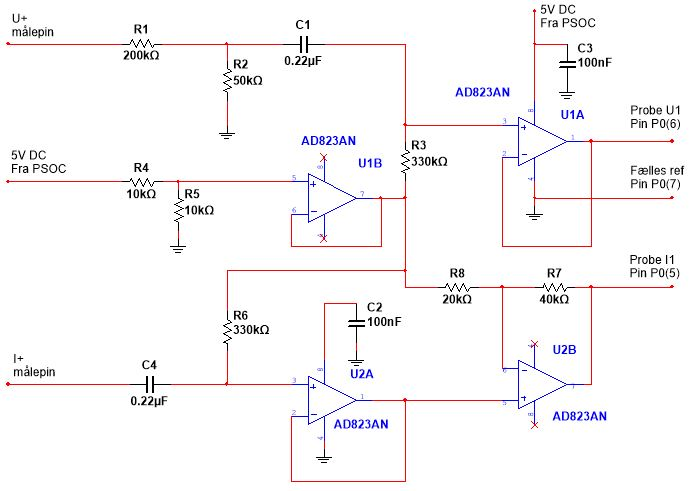
\includegraphics[width=\textwidth]{Figure/MaalHardware}
	\caption{Hardware diagram}
	\label{fig:MaalDiagram}
\end{figure}

